\documentclass{article}
\usepackage[utf8]{inputenc}
\usepackage{amsmath, amssymb, amsfonts, amsthm}
\usepackage{mathtools}
\usepackage{mdframed}
\usepackage{cancel}
\usepackage{import, xifthen, pdfpages, transparent}
\usepackage{enumitem}
\usepackage{geometry}
\usepackage{multicol}
\usepackage{hyperref}
\usepackage{float}
\usepackage{tikz, pgfplots}
\usetikzlibrary{positioning}
\pgfplotsset{compat=1.18}
\geometry{a4paper, margin=2cm}

\newmdenv[
  linecolor=black,
  linewidth=1pt,
  roundcorner=5pt,
  innertopmargin=4pt,
  innerbottommargin=10pt,
  innerleftmargin=10pt,
  innerrightmargin=10pt
]{bxthm}

\theoremstyle{plain}
\newtheorem{thm}{Teorema}[section]
\newtheorem{lem}[thm]{Lemma}
\newtheorem{prop}[thm]{Proposizione}
\newtheorem{cor}{Corollario}

\theoremstyle{definition}
\newtheorem{defn}{Definizione}[section]
\newtheorem{exmp}{Esempio}[section]
\newtheorem{xca}[exmp]{Esercizio}

\theoremstyle{remark}
\newtheorem{rem}{Osservazione}
\newtheorem{note}{Nota}
\newtheorem{case}{Caso}

\newcommand{\incfig}[2][\columnwidth]{%
    \def\svgwidth{#1}
    \import{./figures/}{#2.pdf_tex}
}

\begin{document}

\begin{titlepage}
    \centering
	{\textsc{Università degli Studi della Basilicata} \par}
	\vspace{2cm}
    {\huge\bfseries Appunti rielaborati di Meccanica Razionale 2025/2026\par}
    \vfill
	{\Large\itshape Donato Martinelli\par}
	{\large \today\par}
\end{titlepage}

%\tableofcontents

\newpage 

\section{10-10-25}

\paragraph{Introduzione allo Spazio Affine}

Per descrivere il moto dei corpi, dobbiamo prima definire lo spazio in cui questi si muovono. Introduciamo quindi:

\begin{itemize}
    \item $\mathcal{E}_3$: l'insieme dei punti geometrici dello spazio tridimensionale
    \item $\mathcal{E}_2$: sottoinsieme di $\mathcal{E}_3$ che rappresenta un piano
    \item $\mathcal{E}_1$: sottoinsieme di $\mathcal{E}_3$ che rappresenta una retta
\end{itemize}

\subparagraph{Segmenti Orientati}

Considerando due punti $A,B \in \mathcal{E}_3$, definiamo \emph{segmento orientato} il segmento che li unisce con verso da $A$ a $B$, indicato con $\overrightarrow{AB}$.

\begin{center}
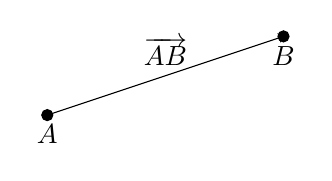
\begin{tikzpicture}
    \draw[->] (0,0) -- (3,1) node[midway, above] {$\overrightarrow{AB}$};
    \filldraw (0,0) circle (2pt) node[below] {$A$};
    \filldraw (3,1) circle (2pt) node[below] {$B$};
\end{tikzpicture}
\end{center}

\subparagraph{Spazio Vettoriale $\mathbf{E}_3$}

Parallelamente, consideriamo lo spazio vettoriale $\mathbf{E}_3$ dei vettori $\mathbf{x}$, che è propriamente euclideo, ovvero:
\[ \|\mathbf{x}\|^2 \geq 0 \quad \forall\,\mathbf{x}\in\mathbf{E}_3 \]
\[ \|\mathbf{x}\|^2 = 0 \iff \mathbf{x}=\mathbf{0} \]

\subparagraph{Spazio Puntuale Affine}

Diciamo che $\mathcal{E}_3$ è uno \emph{spazio puntuale affine propriamente euclideo} se i segmenti orientati soddisfano le seguenti proprietà:

\begin{enumerate}
    \item \textbf{Antisimmetria}: 
    \[ \overrightarrow{AB}=-\overrightarrow{BA} \quad \forall\,A,B\in\mathcal{E}_3 \]
    
    \item \textbf{Regola del parallelogramma}: 
    \[ \overrightarrow{AC}=\overrightarrow{AB}+\overrightarrow{BC} \quad \forall\,A,B,C\in\mathcal{E}_3 \]
    
    \item \textbf{Corrispondenza biunivoca}: 
    \[ \forall O\in\mathcal{E}_3,\forall\mathbf{x}\in\mathbf{E}_3, \exists!P\in\mathcal{E}_3\,:\;\mathbf{x}=\overrightarrow{OP} \]
\end{enumerate}

La terza proprietà stabilisce un'affinità tra i segmenti orientati nello spazio puntuale e i vettori dello spazio vettoriale $\mathbf{E}_3$. Questa corrispondenza biunivoca è fondamentale per poter applicare le proprietà vettoriali ai punti dello spazio.

\subparagraph{Relazione tra Segmenti Orientati e Vettori}

La corrispondenza biunivoca tra segmenti orientati e vettori ci permette di applicare tutte le proprietà vettoriali ai segmenti orientati. In particolare:

\begin{itemize}
    \item Possiamo definire una norma: $\|\overrightarrow{AB}\|^2 \geq 0$
    \item Vale che $\|\overrightarrow{AB}\|^2 = 0$ se e solo se $A = B$
\end{itemize}

Questo ci fornisce uno strumento fondamentale: possiamo applicare ai punti dello spazio affine tutte le proprietà degli spazi vettoriali, pur mantenendo la distinzione concettuale tra punti e vettori.

\subparagraph{Base dello Spazio Vettoriale e Sistema di Riferimento}

Nello spazio vettoriale $\mathbf{E}_3$, possiamo scegliere una base di vettori linearmente indipendenti. Attraverso il processo di ortogonalizzazione di Gram-Schmidt, possiamo ottenere una base ortonormale:

\[\{\mathbf{e}_1, \mathbf{e}_2, \mathbf{e}_3\}\]

\subparagraph{Costruzione del Sistema di Riferimento}

Grazie alla proprietà di corrispondenza biunivoca, possiamo costruire un sistema di riferimento in $\mathcal{E}_3$ seguendo questi passi:

\begin{enumerate}
    \item Scegliamo un punto $O$ (origine) in $\mathcal{E}_3$
    \item Costruiamo tre segmenti orientati partendo da $O$, corrispondenti ai tre versori $\mathbf{e}_1, \mathbf{e}_2, \mathbf{e}_3$
    \item Questi tre segmenti definiscono gli assi coordinati del nostro sistema
\end{enumerate}

\begin{center}
\begin{tikzpicture}[x={(-0.5cm,-0.5cm)}, y={(1cm,0cm)}, z={(0cm,1cm)}]
    % Assi
    \draw[->] (0,0,0) -- (2,0,0) node[right] {$\mathbf{e}_1$};
    \draw[->] (0,0,0) -- (0,2,0) node[right] {$\mathbf{e}_2$};
    \draw[->] (0,0,0) -- (0,0,2) node[above] {$\mathbf{e}_3$};
    % Origine
    \filldraw (0,0,0) circle (1pt) node[below left] {$O$};
\end{tikzpicture}
\end{center}

\subparagraph{Rappresentazione dei Punti}

In questo sistema di riferimento, ogni punto $P$ dello spazio può essere rappresentato attraverso un vettore $\mathbf{x}$ corrispondente al segmento orientato $\overrightarrow{OP}$. Questo vettore si può esprimere come combinazione lineare dei versori di base:
% inserisci figura 1 
\[\mathbf{x} = x_1\mathbf{e}_1 + x_2\mathbf{e}_2 + x_3\mathbf{e}_3\]

dove $x_1, x_2, x_3$ sono le coordinate del punto $P$ rispetto al sistema di riferimento scelto.

\subparagraph{Coordinate di un Punto}

Dato un punto $P$ nello spazio, possiamo identificarne la posizione attraverso le sue coordinate $(x_1,x_2,x_3)$. Queste coordinate, dette rettilinee, si ottengono nel seguente modo:

\begin{enumerate}
    \item Consideriamo il vettore $\overrightarrow{OP}$ che va dall'origine $O$ al punto $P$
    \item Proiettiamo ortogonalmente il punto $P$ sugli assi coordinati
    \item Le coordinate $x_1$, $x_2$, $x_3$ sono le distanze algebriche delle proiezioni dall'origine
\end{enumerate}

\begin{center}
\begin{tikzpicture}[x={(-0.5cm,-0.5cm)}, y={(1cm,0cm)}, z={(0cm,1cm)}]
    % Assi
    \draw[->] (0,0,0) -- (3,0,0) node[right] {$x_1$};
    \draw[->] (0,0,0) -- (0,3,0) node[right] {$x_2$};
    \draw[->] (0,0,0) -- (0,0,3) node[above] {$x_3$};
    % Punto P e sue proiezioni
    \coordinate (P) at (2,1.5,2);
    \filldraw (P) circle (2pt) node[above right] {$P$};
    % Linee tratteggiate per le proiezioni
    \draw[dashed] (P) -- (2,1.5,0);
    \draw[dashed] (P) -- (2,0,2);
    \draw[dashed] (P) -- (0,1.5,2);
    % Origine
    \filldraw (0,0,0) circle (1pt) node[below left] {$O$};
\end{tikzpicture}
\end{center}

Questo sistema di coordinate è chiamato "rettilineo" proprio perché le coordinate sono ottenute mediante proiezioni ortogonali lungo rette (gli assi coordinati).

Grazie a questa costruzione, stabiliamo una corrispondenza biunivoca tra:
\begin{itemize}
    \item I punti dello spazio affine $\mathcal{E}_3$
    \item Le terne ordinate di numeri reali $(x_1,x_2,x_3)$
    \item I vettori dello spazio vettoriale $\mathbf{E}_3$
\end{itemize}

Questo significa che se io prendo due punti $A(x_1,x_2,x_3)$ e $B(z_1,z_2,z_3)$

Riprendi da 24:16



\end{document}
